% GENERATED by tools/to_tmlr.py from main.tex and sections/ (do not edit; edit the sources and regenerate).
\documentclass[10pt]{article}
\usepackage{tmlr}
\usepackage{hyperref}
\DeclareUnicodeCharacter{266B}{}
\DeclareUnicodeCharacter{03C4}{$\tau$}
\newsavebox\fitwidthbox
\newcommand{\fitwidth}[1]{\sbox\fitwidthbox{#1}\ifdim\wd\fitwidthbox>\linewidth\resizebox{\linewidth}{!}{\usebox\fitwidthbox}\else\usebox\fitwidthbox\fi}
\usepackage{amsmath,amssymb,amsthm,booktabs,graphicx,url,xspace,xcolor}
\usepackage{tikz}
\newtheorem{definition}{Definition}
\newtheorem{theorem}{Theorem}
\newtheorem{proposition}{Proposition}
\IfFileExists{generated/numbers.tex}{\RequirePackage{xspace}
% GENERATED by code/scripts/export_paper_numbers.py from results/processed/numbers.json. Do not edit.
\newcommand{\RAubcFactsAdditive}{0.543\xspace}  % aubc.csv
\newcommand{\RAubcFactsAdditiveHi}{0.637\xspace}  % aubc.csv
\newcommand{\RAubcFactsAdditiveLo}{0.448\xspace}  % aubc.csv
\newcommand{\RAubcFactsCov}{0.542\xspace}  % aubc.csv
\newcommand{\RAubcFactsCovHi}{0.628\xspace}  % aubc.csv
\newcommand{\RAubcFactsCovLo}{0.453\xspace}  % aubc.csv
\newcommand{\RAubcFactsFull}{0.580\xspace}  % aubc.csv
\newcommand{\RAubcFactsFullHi}{0.680\xspace}  % aubc.csv
\newcommand{\RAubcFactsFullLo}{0.480\xspace}  % aubc.csv
\newcommand{\RAubcFactsLingua}{0.556\xspace}  % aubc.csv
\newcommand{\RAubcFactsLinguaHi}{0.706\xspace}  % aubc.csv
\newcommand{\RAubcFactsLinguaLo}{0.406\xspace}  % aubc.csv
\newcommand{\RAubcFactsOurs}{0.550\xspace}  % aubc.csv
\newcommand{\RAubcFactsOursHi}{0.645\xspace}  % aubc.csv
\newcommand{\RAubcFactsOursLo}{0.455\xspace}  % aubc.csv
\newcommand{\RAubcFactsRel}{0.575\xspace}  % aubc.csv
\newcommand{\RAubcFactsRelHi}{0.667\xspace}  % aubc.csv
\newcommand{\RAubcFactsRelLo}{0.480\xspace}  % aubc.csv
\newcommand{\RAubcFactsTier}{0.544\xspace}  % aubc.csv
\newcommand{\RAubcFactsTierHi}{0.694\xspace}  % aubc.csv
\newcommand{\RAubcFactsTierLo}{0.394\xspace}  % aubc.csv
\newcommand{\RAubcFactsTrunc}{0.511\xspace}  % aubc.csv
\newcommand{\RAubcFactsTruncHi}{0.650\xspace}  % aubc.csv
\newcommand{\RAubcFactsTruncLo}{0.372\xspace}  % aubc.csv
\newcommand{\RAubcHistoryAdditive}{0.937\xspace}  % aubc.csv
\newcommand{\RAubcHistoryAdditiveHi}{0.953\xspace}  % aubc.csv
\newcommand{\RAubcHistoryAdditiveLo}{0.918\xspace}  % aubc.csv
\newcommand{\RAubcHistoryCov}{0.817\xspace}  % aubc.csv
\newcommand{\RAubcHistoryCovHi}{0.857\xspace}  % aubc.csv
\newcommand{\RAubcHistoryCovLo}{0.773\xspace}  % aubc.csv
\newcommand{\RAubcHistoryFull}{1.000\xspace}  % aubc.csv
\newcommand{\RAubcHistoryFullHi}{1.000\xspace}  % aubc.csv
\newcommand{\RAubcHistoryFullLo}{1.000\xspace}  % aubc.csv
\newcommand{\RAubcHistoryLingua}{0.922\xspace}  % aubc.csv
\newcommand{\RAubcHistoryLinguaHi}{0.950\xspace}  % aubc.csv
\newcommand{\RAubcHistoryLinguaLo}{0.894\xspace}  % aubc.csv
\newcommand{\RAubcHistoryOurs}{0.937\xspace}  % aubc.csv
\newcommand{\RAubcHistoryOursHi}{0.953\xspace}  % aubc.csv
\newcommand{\RAubcHistoryOursLo}{0.918\xspace}  % aubc.csv
\newcommand{\RAubcHistoryRel}{0.990\xspace}  % aubc.csv
\newcommand{\RAubcHistoryRelHi}{0.997\xspace}  % aubc.csv
\newcommand{\RAubcHistoryRelLo}{0.982\xspace}  % aubc.csv
\newcommand{\RAubcHistoryTier}{0.950\xspace}  % aubc.csv
\newcommand{\RAubcHistoryTierHi}{0.978\xspace}  % aubc.csv
\newcommand{\RAubcHistoryTierLo}{0.922\xspace}  % aubc.csv
\newcommand{\RAubcHistoryTrunc}{0.950\xspace}  % aubc.csv
\newcommand{\RAubcHistoryTruncHi}{0.978\xspace}  % aubc.csv
\newcommand{\RAubcHistoryTruncLo}{0.922\xspace}  % aubc.csv
\newcommand{\RAubcToolAdditive}{0.910\xspace}  % aubc.csv
\newcommand{\RAubcToolAdditiveHi}{0.960\xspace}  % aubc.csv
\newcommand{\RAubcToolAdditiveLo}{0.852\xspace}  % aubc.csv
\newcommand{\RAubcToolCov}{0.820\xspace}  % aubc.csv
\newcommand{\RAubcToolCovHi}{0.878\xspace}  % aubc.csv
\newcommand{\RAubcToolCovLo}{0.758\xspace}  % aubc.csv
\newcommand{\RAubcToolFull}{0.900\xspace}  % aubc.csv
\newcommand{\RAubcToolFullHi}{0.950\xspace}  % aubc.csv
\newcommand{\RAubcToolFullLo}{0.840\xspace}  % aubc.csv
\newcommand{\RAubcToolLingua}{0.494\xspace}  % aubc.csv
\newcommand{\RAubcToolLinguaHi}{0.567\xspace}  % aubc.csv
\newcommand{\RAubcToolLinguaLo}{0.422\xspace}  % aubc.csv
\newcommand{\RAubcToolOurs}{0.912\xspace}  % aubc.csv
\newcommand{\RAubcToolOursHi}{0.962\xspace}  % aubc.csv
\newcommand{\RAubcToolOursLo}{0.852\xspace}  % aubc.csv
\newcommand{\RAubcToolRel}{0.905\xspace}  % aubc.csv
\newcommand{\RAubcToolRelHi}{0.957\xspace}  % aubc.csv
\newcommand{\RAubcToolRelLo}{0.848\xspace}  % aubc.csv
\newcommand{\RAubcToolTier}{0.672\xspace}  % aubc.csv
\newcommand{\RAubcToolTierHi}{0.756\xspace}  % aubc.csv
\newcommand{\RAubcToolTierLo}{0.583\xspace}  % aubc.csv
\newcommand{\RAubcToolTrunc}{0.617\xspace}  % aubc.csv
\newcommand{\RAubcToolTruncHi}{0.700\xspace}  % aubc.csv
\newcommand{\RAubcToolTruncLo}{0.528\xspace}  % aubc.csv
\newcommand{\RBaseEightFacts}{55\%\xspace}  % profiles.csv
\newcommand{\RBaseEightHistory}{100\%\xspace}  % profiles.csv
\newcommand{\RBaseEightTool}{85\%\xspace}  % profiles.csv
\newcommand{\RBaseFourFacts}{52\%\xspace}  % profiles.csv
\newcommand{\RBaseFourHistory}{100\%\xspace}  % profiles.csv
\newcommand{\RBaseFourTool}{85\%\xspace}  % profiles.csv
\newcommand{\RBreakEvenFacts}{1{,}016\xspace}  % cost.csv
\newcommand{\RBreakEvenHistory}{5{,}901\xspace}  % cost.csv
\newcommand{\RBreakEvenTool}{931\xspace}  % cost.csv
\newcommand{\RBudgetedEpisodes}{6{,}201\xspace}  % success.csv
\newcommand{\RCoefLen}{0.13\xspace}  % history value model
\newcommand{\RCoefRecency}{0.10\xspace}  % history value model
\newcommand{\RCoefSim}{0.34\xspace}  % history value model
\newcommand{\RCoverage}{96\%\xspace}  % coverage.json
\newcommand{\RCvModelFacts}{0.07\xspace}  % value_model_cv.csv
\newcommand{\RCvModelHistory}{0.15\xspace}  % value_model_cv.csv
\newcommand{\RCvModelTool}{0.27\xspace}  % value_model_cv.csv
\newcommand{\RCvNFacts}{215\xspace}  % value_model_cv.csv
\newcommand{\RCvNHistory}{219\xspace}  % value_model_cv.csv
\newcommand{\RCvNTool}{217\xspace}  % value_model_cv.csv
\newcommand{\RCvNonzeroFacts}{5\%\xspace}  % value_model_cv.csv
\newcommand{\RCvNonzeroHistory}{5\%\xspace}  % value_model_cv.csv
\newcommand{\RCvNonzeroTool}{4\%\xspace}  % value_model_cv.csv
\newcommand{\RCvSimFacts}{0.17\xspace}  % value_model_cv.csv
\newcommand{\RCvSimHistory}{0.27\xspace}  % value_model_cv.csv
\newcommand{\RCvSimTool}{0.27\xspace}  % value_model_cv.csv
\newcommand{\RDevAubcOne}{0.633\xspace}  % pilot_dev_4b (OURS, mean over families)
\newcommand{\RDevAubcThree}{0.736\xspace}  % pilot3_dev_4b (OURS, mean over families)
\newcommand{\RDevAubcTwo}{0.758\xspace}  % pilot2_dev_4b (OURS, mean over families)
\newcommand{\RFactsGained}{2\xspace}  % facts 8k: OURS correct, B0 wrong
\newcommand{\RFactsLost}{6\xspace}  % facts 8k: B0 correct, OURS wrong
\newcommand{\RFactsLostGoldDropped}{2\xspace}  % facts 8k losses with a supporting paragraph removed
\newcommand{\RFullTokFacts}{2{,}961\xspace}  % instances.jsonl (mean full-context tokens)
\newcommand{\RFullTokHistory}{2{,}718\xspace}  % instances.jsonl (mean full-context tokens)
\newcommand{\RFullTokTool}{4{,}235\xspace}  % instances.jsonl (mean full-context tokens)
\newcommand{\RHOneFactsDiff}{-0.025\xspace}  % tests.csv
\newcommand{\RHOneFactsHi}{0.018\xspace}  % tests.csv
\newcommand{\RHOneFactsLo}{-0.070\xspace}  % tests.csv
\newcommand{\RHOneFactsP}{1.000\xspace}  % tests.csv
\newcommand{\RHOneHistoryDiff}{-0.053\xspace}  % tests.csv
\newcommand{\RHOneHistoryHi}{-0.035\xspace}  % tests.csv
\newcommand{\RHOneHistoryLo}{-0.072\xspace}  % tests.csv
\newcommand{\RHOneHistoryP}{0.000\xspace}  % tests.csv
\newcommand{\RHOneToolDiff}{0.007\xspace}  % tests.csv
\newcommand{\RHOneToolHi}{0.027\xspace}  % tests.csv
\newcommand{\RHOneToolLo}{-0.012\xspace}  % tests.csv
\newcommand{\RHOneToolP}{1.000\xspace}  % tests.csv
\newcommand{\RHOnebFactsDiff}{-0.040\xspace}  % tests.csv
\newcommand{\RHOnebFactsHi}{0.010\xspace}  % tests.csv
\newcommand{\RHOnebFactsLo}{-0.100\xspace}  % tests.csv
\newcommand{\RHOnebFactsP}{1.000\xspace}  % tests.csv
\newcommand{\RHOnebHistoryDiff}{0.000\xspace}  % tests.csv
\newcommand{\RHOnebHistoryHi}{0.000\xspace}  % tests.csv
\newcommand{\RHOnebHistoryLo}{0.000\xspace}  % tests.csv
\newcommand{\RHOnebHistoryP}{0.001\xspace}  % tests.csv
\newcommand{\RHOnebPass}{2\xspace}  % h1b.csv
\newcommand{\RHOnebToolDiff}{0.010\xspace}  % tests.csv
\newcommand{\RHOnebToolHi}{0.030\xspace}  % tests.csv
\newcommand{\RHOnebToolLo}{0.000\xspace}  % tests.csv
\newcommand{\RHOnebToolP}{0.001\xspace}  % tests.csv
\newcommand{\RHThreeVerdict}{non-inferior\xspace}  % transfer runs: lower CI bound vs margin
\newcommand{\RHTwoPooledDiff}{0.003\xspace}  % tests.csv
\newcommand{\RHTwoPooledHi}{0.007\xspace}  % tests.csv
\newcommand{\RHTwoPooledLo}{-0.001\xspace}  % tests.csv
\newcommand{\RHTwoPooledP}{1.000\xspace}  % tests.csv
\newcommand{\RIntFactsExampleFact}{0.10\xspace}  % profiles.csv
\newcommand{\RIntHistoryExampleHistoryTurn}{0.00\xspace}  % profiles.csv
\newcommand{\RIntHistoryExampleNote}{0.00\xspace}  % profiles.csv
\newcommand{\RIntHistoryHistoryTurnNote}{-0.60\xspace}  % profiles.csv
\newcommand{\RIntToolExampleToolSchema}{0.03\xspace}  % profiles.csv
\newcommand{\RLoc}{1{,}227\xspace}  % code/mcv non-blank lines
\newcommand{\RMainEpisodes}{6{,}180\xspace}  % main_4b + main_4b_weak
\newcommand{\RMargin}{0.05\xspace}  % PLAN.md
\newcommand{\RMaxOvershoot}{2\xspace}  % max measured prompt minus budget
\newcommand{\RMcvEightFactsExample}{0.00\xspace}  % profiles.csv
\newcommand{\RMcvEightFactsFact}{0.35\xspace}  % profiles.csv
\newcommand{\RMcvEightHistoryExample}{0.10\xspace}  % profiles.csv
\newcommand{\RMcvEightHistoryHistoryTurn}{0.45\xspace}  % profiles.csv
\newcommand{\RMcvEightHistoryNote}{0.05\xspace}  % profiles.csv
\newcommand{\RMcvEightToolExample}{-0.05\xspace}  % profiles.csv
\newcommand{\RMcvEightToolToolSchema}{0.80\xspace}  % profiles.csv
\newcommand{\RMcvFactsExample}{0.05\xspace}  % profiles.csv
\newcommand{\RMcvFactsFact}{0.35\xspace}  % profiles.csv
\newcommand{\RMcvHistoryExample}{0.00\xspace}  % profiles.csv
\newcommand{\RMcvHistoryHistoryTurn}{0.40\xspace}  % profiles.csv
\newcommand{\RMcvHistoryNote}{0.00\xspace}  % profiles.csv
\newcommand{\RMcvToolExample}{-0.03\xspace}  % profiles.csv
\newcommand{\RMcvToolToolSchema}{0.85\xspace}  % profiles.csv
\newcommand{\RNBoot}{10{,}000\xspace}  % analysis
\newcommand{\RNDev}{60\xspace}  % instances.jsonl
\newcommand{\RNFactsAdditive}{100\xspace}  % aubc.csv
\newcommand{\RNFactsCov}{100\xspace}  % aubc.csv
\newcommand{\RNFactsFull}{100\xspace}  % aubc.csv
\newcommand{\RNFactsLingua}{30\xspace}  % aubc.csv
\newcommand{\RNFactsOurs}{100\xspace}  % aubc.csv
\newcommand{\RNFactsRel}{100\xspace}  % aubc.csv
\newcommand{\RNFactsTier}{30\xspace}  % aubc.csv
\newcommand{\RNFactsTrunc}{30\xspace}  % aubc.csv
\newcommand{\RNHistoryAdditive}{100\xspace}  % aubc.csv
\newcommand{\RNHistoryCov}{100\xspace}  % aubc.csv
\newcommand{\RNHistoryFull}{100\xspace}  % aubc.csv
\newcommand{\RNHistoryLingua}{30\xspace}  % aubc.csv
\newcommand{\RNHistoryOurs}{100\xspace}  % aubc.csv
\newcommand{\RNHistoryRel}{100\xspace}  % aubc.csv
\newcommand{\RNHistoryTier}{30\xspace}  % aubc.csv
\newcommand{\RNHistoryTrunc}{30\xspace}  % aubc.csv
\newcommand{\RNLobo}{6\xspace}  % mcv/run.py --lobo default
\newcommand{\RNMain}{100\xspace}  % experiments/run_all.sh --limit (main grid)
\newcommand{\RNPerFamily}{300\xspace}  % mcv/data/build.py
\newcommand{\RNProfEight}{20\xspace}  % profiles.csv
\newcommand{\RNProfFour}{40\xspace}  % profiles.csv
\newcommand{\RNTest}{240\xspace}  % instances.jsonl
\newcommand{\RNToolAdditive}{100\xspace}  % aubc.csv
\newcommand{\RNToolCov}{100\xspace}  % aubc.csv
\newcommand{\RNToolFull}{100\xspace}  % aubc.csv
\newcommand{\RNToolLingua}{30\xspace}  % aubc.csv
\newcommand{\RNToolOurs}{100\xspace}  % aubc.csv
\newcommand{\RNToolRel}{100\xspace}  % aubc.csv
\newcommand{\RNToolTier}{30\xspace}  % aubc.csv
\newcommand{\RNToolTrunc}{30\xspace}  % aubc.csv
\newcommand{\RNTransfer}{40\xspace}  % experiments/run_all.sh --limit (transfer)
\newcommand{\RNWeak}{30\xspace}  % experiments/run_all.sh --limit (weak baselines)
\newcommand{\RNZero}{10\xspace}  % mcv/profile/estimate.py
\newcommand{\RNumCtx}{16{,}384\xspace}  % mcv/agent/loop.py
\newcommand{\RNumDocs}{20\xspace}  % instances.jsonl
\newcommand{\RNumPredict}{96\xspace}  % mcv/agent/loop.py num_predict
\newcommand{\RNumSessions}{24\xspace}  % instances.jsonl
\newcommand{\RNumTools}{30\xspace}  % instances.jsonl
\newcommand{\ROllamaVersion}{0.35.0\xspace}  % ENVIRONMENT.md
\newcommand{\ROverBudget}{34\xspace}  % success.csv (budgeted episodes with measured prompt > budget)
\newcommand{\RPadDiffMax}{0.05\xspace}  % padding.csv
\newcommand{\RPadFactsExample}{0.00\xspace}  % padding.csv
\newcommand{\RPadFactsFact}{0.45\xspace}  % padding.csv
\newcommand{\RPadHistoryExample}{0.00\xspace}  % padding.csv
\newcommand{\RPadHistoryHistoryTurn}{0.45\xspace}  % padding.csv
\newcommand{\RPadHistoryNote}{0.00\xspace}  % padding.csv
\newcommand{\RPadN}{20\xspace}  % padding.csv
\newcommand{\RPadToolExample}{0.00\xspace}  % padding.csv
\newcommand{\RPadToolToolSchema}{0.90\xspace}  % padding.csv
\newcommand{\RPlanMedianMs}{6.9\xspace}  % plan_seconds
\newcommand{\RPowerFacts}{58\%\xspace}  % PLAN.md power analysis (facts, n = 100)
\newcommand{\RProfCallsFacts}{440\xspace}  % cost.csv
\newcommand{\RProfCallsHistory}{560\xspace}  % cost.csv
\newcommand{\RProfCallsTool}{440\xspace}  % cost.csv
\newcommand{\RProfCallsTotal}{1{,}440\xspace}  % cost.csv
\newcommand{\RProfHours}{3.0\xspace}  % cost.csv
\newcommand{\RRecallAdditive}{64\%\xspace}  % history_recall.csv
\newcommand{\RRecallCov}{20\%\xspace}  % history_recall.csv
\newcommand{\RRecallLingua}{0\%\xspace}  % history_recall.csv
\newcommand{\RRecallOurs}{64\%\xspace}  % history_recall.csv
\newcommand{\RRecallRel}{94\%\xspace}  % history_recall.csv
\newcommand{\RRecallTier}{43\%\xspace}  % history_recall.csv
\newcommand{\RRecallTrunc}{43\%\xspace}  % history_recall.csv
\newcommand{\RRemFactsExample}{0.00\xspace}  % padding.csv
\newcommand{\RRemFactsFact}{0.50\xspace}  % padding.csv
\newcommand{\RRemHistoryExample}{0.00\xspace}  % padding.csv
\newcommand{\RRemHistoryHistoryTurn}{0.45\xspace}  % padding.csv
\newcommand{\RRemHistoryNote}{0.00\xspace}  % padding.csv
\newcommand{\RRemToolExample}{0.00\xspace}  % padding.csv
\newcommand{\RRemToolToolSchema}{0.90\xspace}  % padding.csv
\newcommand{\RRho}{0.88\xspace}  % fidelity.csv
\newcommand{\RRhoN}{7\xspace}  % fidelity.csv
\newcommand{\RScale}{10{,}000\xspace}  % mcv/compile/knapsack.py
\newcommand{\RSesoi}{0.05\xspace}  % PLAN.md power analysis (smallest effect of interest)
\newcommand{\RShortFactsFact}{0.12\xspace}  % profiles.csv
\newcommand{\RShortHistoryHistoryTurn}{-0.03\xspace}  % profiles.csv
\newcommand{\RShortToolToolSchema}{0.30\xspace}  % profiles.csv
\newcommand{\RSolveFallback}{0\xspace}  % certificates
\newcommand{\RSolveMaxMs}{357\xspace}  % certificates
\newcommand{\RSolveMedianMs}{2.3\xspace}  % certificates
\newcommand{\RSolveNinetyNineMs}{22.3\xspace}  % certificates
\newcommand{\RSolveOptimal}{100.0\%\xspace}  % certificates
\newcommand{\RSolves}{2{,}400\xspace}  % certificates
\newcommand{\RSsDraws}{300\xspace}  % analyze_profiles.py
\newcommand{\RSsMaeFive}{0.09\xspace}  % profile_sample_size.csv
\newcommand{\RSsMaeTen}{0.06\xspace}  % profile_sample_size.csv
\newcommand{\RSsMaeThirty}{0.02\xspace}  % profile_sample_size.csv
\newcommand{\RSsMaeTwenty}{0.03\xspace}  % profile_sample_size.csv
\newcommand{\RSsRhoFive}{0.90\xspace}  % profile_sample_size.csv
\newcommand{\RSsRhoTen}{0.93\xspace}  % profile_sample_size.csv
\newcommand{\RSsRhoThirty}{0.99\xspace}  % profile_sample_size.csv
\newcommand{\RSsRhoTwenty}{0.97\xspace}  % profile_sample_size.csv
\newcommand{\RSsTopFive}{74\%\xspace}  % profile_sample_size.csv
\newcommand{\RSsTopTen}{92\%\xspace}  % profile_sample_size.csv
\newcommand{\RSsTopThirty}{100\%\xspace}  % profile_sample_size.csv
\newcommand{\RSsTopTwenty}{99\%\xspace}  % profile_sample_size.csv
\newcommand{\RStatusNotOk}{0\xspace}  % main runs
\newcommand{\RSucFactsAdditiveEight}{54\%\xspace}  % success.csv
\newcommand{\RSucFactsAdditiveFour}{54\%\xspace}  % success.csv
\newcommand{\RSucFactsAdditiveOne}{50\%\xspace}  % success.csv
\newcommand{\RSucFactsAdditiveTwo}{57\%\xspace}  % success.csv
\newcommand{\RSucFactsCovEight}{58\%\xspace}  % success.csv
\newcommand{\RSucFactsCovFour}{58\%\xspace}  % success.csv
\newcommand{\RSucFactsCovOne}{45\%\xspace}  % success.csv
\newcommand{\RSucFactsCovTwo}{53\%\xspace}  % success.csv
\newcommand{\RSucFactsLinguaEight}{63\%\xspace}  % success.csv
\newcommand{\RSucFactsLinguaFour}{63\%\xspace}  % success.csv
\newcommand{\RSucFactsLinguaOne}{37\%\xspace}  % success.csv
\newcommand{\RSucFactsLinguaTwo}{53\%\xspace}  % success.csv
\newcommand{\RSucFactsOursEight}{54\%\xspace}  % success.csv
\newcommand{\RSucFactsOursFour}{54\%\xspace}  % success.csv
\newcommand{\RSucFactsOursOne}{54\%\xspace}  % success.csv
\newcommand{\RSucFactsOursTwo}{57\%\xspace}  % success.csv
\newcommand{\RSucFactsRelEight}{58\%\xspace}  % success.csv
\newcommand{\RSucFactsRelFour}{58\%\xspace}  % success.csv
\newcommand{\RSucFactsRelOne}{57\%\xspace}  % success.csv
\newcommand{\RSucFactsRelTwo}{57\%\xspace}  % success.csv
\newcommand{\RSucFactsTierEight}{63\%\xspace}  % success.csv
\newcommand{\RSucFactsTierFour}{63\%\xspace}  % success.csv
\newcommand{\RSucFactsTierOne}{30\%\xspace}  % success.csv
\newcommand{\RSucFactsTierTwo}{53\%\xspace}  % success.csv
\newcommand{\RSucFactsTruncEight}{63\%\xspace}  % success.csv
\newcommand{\RSucFactsTruncFour}{63\%\xspace}  % success.csv
\newcommand{\RSucFactsTruncOne}{23\%\xspace}  % success.csv
\newcommand{\RSucFactsTruncTwo}{47\%\xspace}  % success.csv
\newcommand{\RSucFullFacts}{58\%\xspace}  % h1b.csv
\newcommand{\RSucFullHistory}{100\%\xspace}  % h1b.csv
\newcommand{\RSucFullTool}{90\%\xspace}  % h1b.csv
\newcommand{\RSucGivenNoGoldOurs}{0\%\xspace}  % history_recall.csv
\newcommand{\RSucHistoryAdditiveEight}{100\%\xspace}  % success.csv
\newcommand{\RSucHistoryAdditiveFour}{100\%\xspace}  % success.csv
\newcommand{\RSucHistoryAdditiveOne}{64\%\xspace}  % success.csv
\newcommand{\RSucHistoryAdditiveTwo}{99\%\xspace}  % success.csv
\newcommand{\RSucHistoryCovEight}{100\%\xspace}  % success.csv
\newcommand{\RSucHistoryCovFour}{100\%\xspace}  % success.csv
\newcommand{\RSucHistoryCovOne}{54\%\xspace}  % success.csv
\newcommand{\RSucHistoryCovTwo}{68\%\xspace}  % success.csv
\newcommand{\RSucHistoryLinguaEight}{100\%\xspace}  % success.csv
\newcommand{\RSucHistoryLinguaFour}{100\%\xspace}  % success.csv
\newcommand{\RSucHistoryLinguaOne}{53\%\xspace}  % success.csv
\newcommand{\RSucHistoryLinguaTwo}{100\%\xspace}  % success.csv
\newcommand{\RSucHistoryOursEight}{100\%\xspace}  % success.csv
\newcommand{\RSucHistoryOursFour}{100\%\xspace}  % success.csv
\newcommand{\RSucHistoryOursOne}{64\%\xspace}  % success.csv
\newcommand{\RSucHistoryOursTwo}{99\%\xspace}  % success.csv
\newcommand{\RSucHistoryRelEight}{100\%\xspace}  % success.csv
\newcommand{\RSucHistoryRelFour}{100\%\xspace}  % success.csv
\newcommand{\RSucHistoryRelOne}{94\%\xspace}  % success.csv
\newcommand{\RSucHistoryRelTwo}{100\%\xspace}  % success.csv
\newcommand{\RSucHistoryTierEight}{100\%\xspace}  % success.csv
\newcommand{\RSucHistoryTierFour}{100\%\xspace}  % success.csv
\newcommand{\RSucHistoryTierOne}{70\%\xspace}  % success.csv
\newcommand{\RSucHistoryTierTwo}{100\%\xspace}  % success.csv
\newcommand{\RSucHistoryTruncEight}{100\%\xspace}  % success.csv
\newcommand{\RSucHistoryTruncFour}{100\%\xspace}  % success.csv
\newcommand{\RSucHistoryTruncOne}{70\%\xspace}  % success.csv
\newcommand{\RSucHistoryTruncTwo}{100\%\xspace}  % success.csv
\newcommand{\RSucOursEightFacts}{54\%\xspace}  % h1b.csv
\newcommand{\RSucOursEightHistory}{100\%\xspace}  % h1b.csv
\newcommand{\RSucOursEightTool}{91\%\xspace}  % h1b.csv
\newcommand{\RSucToolAdditiveEight}{91\%\xspace}  % success.csv
\newcommand{\RSucToolAdditiveFour}{91\%\xspace}  % success.csv
\newcommand{\RSucToolAdditiveOne}{91\%\xspace}  % success.csv
\newcommand{\RSucToolAdditiveTwo}{91\%\xspace}  % success.csv
\newcommand{\RSucToolCovEight}{90\%\xspace}  % success.csv
\newcommand{\RSucToolCovFour}{89\%\xspace}  % success.csv
\newcommand{\RSucToolCovOne}{62\%\xspace}  % success.csv
\newcommand{\RSucToolCovTwo}{81\%\xspace}  % success.csv
\newcommand{\RSucToolLinguaEight}{97\%\xspace}  % success.csv
\newcommand{\RSucToolLinguaFour}{83\%\xspace}  % success.csv
\newcommand{\RSucToolLinguaOne}{0\%\xspace}  % success.csv
\newcommand{\RSucToolLinguaTwo}{17\%\xspace}  % success.csv
\newcommand{\RSucToolOursEight}{91\%\xspace}  % success.csv
\newcommand{\RSucToolOursFour}{91\%\xspace}  % success.csv
\newcommand{\RSucToolOursOne}{92\%\xspace}  % success.csv
\newcommand{\RSucToolOursTwo}{91\%\xspace}  % success.csv
\newcommand{\RSucToolRelEight}{90\%\xspace}  % success.csv
\newcommand{\RSucToolRelFour}{90\%\xspace}  % success.csv
\newcommand{\RSucToolRelOne}{91\%\xspace}  % success.csv
\newcommand{\RSucToolRelTwo}{91\%\xspace}  % success.csv
\newcommand{\RSucToolTierEight}{97\%\xspace}  % success.csv
\newcommand{\RSucToolTierFour}{97\%\xspace}  % success.csv
\newcommand{\RSucToolTierOne}{20\%\xspace}  % success.csv
\newcommand{\RSucToolTierTwo}{47\%\xspace}  % success.csv
\newcommand{\RSucToolTruncEight}{97\%\xspace}  % success.csv
\newcommand{\RSucToolTruncFour}{90\%\xspace}  % success.csv
\newcommand{\RSucToolTruncOne}{7\%\xspace}  % success.csv
\newcommand{\RSucToolTruncTwo}{43\%\xspace}  % success.csv
\newcommand{\RTests}{18\xspace}  % tests.xml
\newcommand{\RTimeLimit}{2.0\xspace}  % mcv/compile/knapsack.py
\newcommand{\RTokCutFacts}{30.9\%\xspace}  % h1b.csv
\newcommand{\RTokCutHistory}{6.9\%\xspace}  % h1b.csv
\newcommand{\RTokCutTool}{34.9\%\xspace}  % h1b.csv
\newcommand{\RTokFullFacts}{2{,}998\xspace}  % h1b.csv
\newcommand{\RTokFullHistory}{2{,}717\xspace}  % h1b.csv
\newcommand{\RTokFullTool}{4{,}240\xspace}  % h1b.csv
\newcommand{\RTokOursFacts}{2{,}072\xspace}  % h1b.csv
\newcommand{\RTokOursHistory}{2{,}529\xspace}  % h1b.csv
\newcommand{\RTokOursTool}{2{,}759\xspace}  % h1b.csv
\newcommand{\RTrFactsNativeEight}{62\%\xspace}  % transfer.csv
\newcommand{\RTrFactsNativeTwo}{62\%\xspace}  % transfer.csv
\newcommand{\RTrFactsRelEight}{68\%\xspace}  % transfer.csv
\newcommand{\RTrFactsRelTwo}{68\%\xspace}  % transfer.csv
\newcommand{\RTrFactsTransferEight}{62\%\xspace}  % transfer.csv
\newcommand{\RTrFactsTransferTwo}{62\%\xspace}  % transfer.csv
\newcommand{\RTrHistoryRelEight}{98\%\xspace}  % transfer.csv
\newcommand{\RTrHistoryRelTwo}{98\%\xspace}  % transfer.csv
\newcommand{\RTrHistoryTransferEight}{100\%\xspace}  % transfer.csv
\newcommand{\RTrHistoryTransferTwo}{100\%\xspace}  % transfer.csv
\newcommand{\RTrN}{18\xspace}  % transfer.csv
\newcommand{\RTransferDiff}{0.000\xspace}  % transfer runs (pooled OURS-T minus OURS-native)
\newcommand{\RTransferHi}{0.000\xspace}  % transfer runs
\newcommand{\RTransferLo}{0.000\xspace}  % transfer runs
\newcommand{\RTransferN}{80\xspace}  % transfer runs
\newcommand{\RTransferSameSel}{74\%\xspace}  % transfer runs: identical selections OURS-T vs OURS-native
}{}

\title{Context That Pays: Ablation-Calibrated Marginal Context Value Profiles for Budgeted Context Assembly}
\author{\name Venkata Sangaraju \email sangaraju1988@gmail.com \\
      \addr Independent Researcher, Leander, TX, USA}
\def\month{MM}
\def\year{YYYY}
\def\openreview{\url{https://openreview.net/forum?id=XXXX}}

\begin{document}
\maketitle
\begin{abstract}
% Numbers via \R macros only.
LLM agents assemble prompts from heterogeneous context (tool schemas, documents, examples, notes, history) under a
token budget. We separate three questions: which context types matter for a model and task family, which blocks matter
for an instance, and what to send under a budget. Marginal context value (MCV) profiles address the first: measured
success drops when a type is removed, short-variant values and type interactions, estimated offline by ablation with
bootstrap intervals. A CP-SAT compiler optimizes predicted block values under budget, dependency and variant
constraints; its certificate covers that objective, not task success. In a pre-registered local evaluation on
Qwen3-4B-Instruct (HotpotQA, BFCL tool calling, synthetic history) the primary hypothesis failed: MCV did not
significantly exceed embedding relevance in any family and trailed it by \RHOneHistoryAbs{} AUBC on history.
Single-block deletions rarely changed outcomes, and the learned block ranker leaned on recency and length and never
beat embedding similarity. At a non-binding 8k budget MCV pruned \RTokCutTool of prompt tokens on tool calling and
\RTokCutHistory on history with non-inferior success. In a pre-specified post-hoc follow-up, relevance with a
calibrated stopping rule pruned \RTokCutStopTool on tool calling with non-inferior success, so these savings are not
specific to MCV, and a hybrid (profile admits types, relevance ranks blocks) beat relevance in no family. Interaction
terms had no detectable effect. As diagnostics the profiles were informative: tool schemas, documents and history
carried most of the value, worked examples little individual value, and shortened tool schemas lost most of theirs. 4B
and 8B type values were rank-correlated ($\rho=\RRho$, \RRhoN pairs), and transferred and native profiles gave
identical paired outcomes, consistent with transfer or with compiler insensitivity. Code and all logs are released.

\end{abstract}
\section{Introduction}\label{sec:intro}
% INTRODUCTION. Numbers ONLY via \R... macros from generated/numbers.tex.
An LLM agent's prompt is assembled, not written. Before each decision a harness collects tool schemas, retrieved
documents, worked examples, notes and conversation history, and must fit them into a token budget set by latency, cost or
the model's window~\citep{cesurvey2025}. What to keep is usually decided by heuristics: a relevance score against the
goal, a coverage objective over candidate passages~\citep{pacms2026}, a compressor that deletes tokens~\citep{llmlingua2_2024},
or fixed priorities written by an engineer. None of these asks the question a budgeted system actually faces:
\emph{how much does this kind of context change task success for this model on this task family?} The answer is not
obvious. Models use long contexts unevenly~\citep{lostmiddle2024}, and a block can be relevant to the goal yet add
nothing the model needs, or be redundant with another block that is already included.

This paper asks: when context consists of heterogeneous types, can we measure how much each type contributes to task
success, and can those measurements be reused for budgeted assembly? We separate three levels of the problem
(Section~\ref{sec:problem}): \emph{type value} (which kinds of context matter for a model and task family),
\emph{block relevance} (which particular blocks matter for an instance), and \emph{budget allocation} (what to send under a
token limit, and when to stop). A \emph{marginal context value (MCV) profile} answers the first level. For a (model, task
family) pair it records the measured drop in success when every block of a type is removed, the value of the type's
short variant, and pairwise interactions between types, each with a bootstrap interval. Profiles are estimated once,
offline, by counterfactual ablation on development instances, with a length-neutral control. For the second level we
train a block-value model on leave-one-block-out deltas from the same runs. For the third, a CP-SAT compiler maximizes
predicted value under the budget, dependencies and variants without calling the language model, and reports a
certificate of optimality for that predicted objective.

Prior work values context in related ways but for other decisions: attribution methods explain one generation by
ablating its sources~\citep{contextcite2024,attribot2024}, Shapley-style methods value demonstrations, prompts, data
points or skills~\citep{demoshapley2024,promptshapley2023,datashapley2019,skillsv2026}, and recent context-allocation
studies measure the causal effect of context in generative search~\citep{ctxalloc2026}. The distinguishing combination is a reusable,
type-level, interval-reported value table measured per model and task family and compiled under a hard token budget.

We evaluate the approach under a pre-registered protocol (hypotheses, margins, sample sizes and the method version fixed
before any test run, recorded as a commit in the released repository; it was not deposited with an external registry) on three task families: multi-hop question answering over HotpotQA documents with distractors,
tool selection and argument filling over a \RNumTools-tool catalog built from BFCL, and recall of the latest value of a
user attribute from \RNumSessions synthetic sessions. All models run locally (Qwen3-4B-Instruct for the main study,
Qwen3-8B for transfer). We compare against six baselines, including LLMLingua-2 and a PACMS-style coverage selector.

The primary result is negative, and we lead with it. \textbf{MCV did not beat relevance at block selection:}
MCV-compiled context did not significantly exceed embedding relevance (the best baseline) in area under the
success--budget curve in any family, and was \RHOneHistoryAbs{} lower on history. The cause is at the block level. Single
deletions rarely change the outcome, so the block-value model learned proxies such as recency and length. At the smallest
history budget it kept the session holding the answer in \RRecallOurs of plans, against \RRecallRel for relevance.
\textbf{Efficiency held, but is not specific to MCV.} The efficiency hypothesis, added after development pilots but before
any test run, held in \RHOnebPass of three families: at an 8k budget, which full contexts never reach, MCV pruned
\RTokCutTool of prompt tokens on tool use and \RTokCutHistory on history with non-inferior success. A pre-specified
post-hoc follow-up showed that relevance with a calibrated stopping rule pruned more (\RTokCutStopTool on tool use, also
non-inferior), and that a hybrid in which the profile admits types and relevance ranks blocks did not beat relevance.
Interaction terms had no detectable effect. \textbf{As a diagnostic, the profiles were informative.} Tool schemas,
documents and history carried most of the value (\RMcvToolToolSchema, \RMcvFactsFact, \RMcvHistoryHistoryTurn),
worked examples little on their own, and shortened tool schemas lost most of theirs. History and the profile note
substituted for each other (interaction \RIntHistoryHistoryTurnNote), and the length-neutral control moved no value by
more than \RPadDiffMax. Qwen3-4B and Qwen3-8B type values were rank-correlated ($\rho=\RRho$), but outcome agreement under
transferred and native profiles may reflect compiler insensitivity as much as transfer.

\textbf{Contributions.}
\begin{itemize}
\item \emph{A three-level view of context assembly} (type value, block relevance, budget allocation), with evidence that
the levels should not be served by one signal: measured type value was informative, while block selection was best served
by embedding relevance (Sections~\ref{sec:problem} and~\ref{sec:eval}).
\item \emph{MCV profiles as a reusable type-level diagnostic:} an estimator of per-(model, family) type values,
short-variant values and interactions with shrinkage, bootstrap intervals and a length-neutral control, with measured
stability (ten to twenty development instances in subsampling), cost and Qwen3-4B-to-8B agreement.
\item \emph{A controlled, pre-registered evaluation} of ten context policies on three task families, including a failed
primary hypothesis, a pre-specified follow-up, and evidence that leave-one-block-out deltas were too sparse to train a
block ranker that improves on embedding similarity.
\item \emph{A dependency- and variant-aware exact budget compiler} whose certificate is bounded to the predicted
objective, not task success (Section~\ref{sec:design}).
\item \emph{An open artifact:} code, data adapters, logs of every model call, and scripts that regenerate every number,
table and figure.
\end{itemize}

\section{Background and Related Work}\label{sec:related}
% BACKGROUND AND RELATED WORK. Claims about prior work are limited to what each paper's abstract or full text states.

\subsection{Context Engineering and Assembly}
A survey formalizes context engineering as the discipline of retrieving, processing and managing the information supplied
to a language model at inference time~\citep{cesurvey2025}. Agentic Context Engineering treats contexts as evolving
playbooks that accumulate and refine strategies~\citep{ace2025}, and DSPy compiles declarative pipelines of language-model
calls into optimized prompts~\citep{dspy2023}; both optimize the \emph{content} of context rather than selecting among
existing blocks under a budget. Several 2026 systems assemble context for long-horizon agents. ContextPipe organizes
assembly as a five-phase, database-style pipeline with a data-source catalog and a cache-aware optimizer, and notes that
maximizing utility under a budget with precedence is a precedence-constrained knapsack that it deliberately does not
search~\citep{contextpipe2026}. ContextRender selects earlier tool results using observed reuse in an execution-dependency
graph together with recency and relevance~\citep{contextrender2026}. Context Assembly as the Controlled Variable frames the
choice of template, demonstrations and retrieval as the variable a harness controls~\citep{controlledvar2026}; ContextEvo
learns a context-management policy from long-horizon trajectories~\citep{contextevo2026}; programmatic context management
treats context as an environment the agent manipulates~\citep{ctxenv2026}; and Imprompt treats prompts as a programmable
control surface~\citep{imprompt2026}. These systems decide what enters context through rules, learned policies or
relevance signals. None measures, ahead of time, what each kind of block is worth to task success.

\subsection{Selection Under a Token Budget}
PACMS casts assembly-time selection as submodular maximum coverage under a knapsack constraint and solves it with a
cost-aware greedy over pluggable selectors~\citep{pacms2026}. Budgeted skill selection has been formulated as regularized
submodular maximization with provable bicriteria guarantees, modelling complementarity through coverage and
diminishing returns; its authors name interaction terms learned from execution feedback as future
work~\citep{skillselect2026}. In retrieval-augmented generation, budget allocation has been approached by calibrated
decisions about how much to retrieve~\citep{knowbefore2026}, by a reader-context diagnostic for budget-constrained
selection~\citep{recallnotenough2026}, by dependency-structured memory selection~\citep{contextweaver2026}, and by
constructing knowledge-base context from historical usage for text-to-SQL~\citep{beyondharness2026}. Tool schemas compete
with retrieved evidence for the same window, which motivates schema compression~\citep{toolschema2026}, and budget-tiered
protocols evaluate memory strategies for local agents~\citep{budgetbench2026}. Long contexts are also used unevenly by
models, which perform worse when relevant information sits in the middle~\citep{lostmiddle2024}.

\subsection{Compression}
LLMLingua-2 distils token-level compression into a small classifier that keeps the tokens a teacher marks as
essential~\citep{llmlingua2_2024}, and COMI compresses context by a marginal-information-gain score that rewards relevance
and penalizes redundancy~\citep{comi2026}. A pre-registered randomized trial of compression in production task orchestration
shows that savings depend on how compression changes output length~\citep{compressiontrial2026}, and compressing the
persistent instructions of tool-using agents traces reliability frontiers~\citep{controlcompression2026}. Compression keeps
every block but shortens it; our compiler instead chooses which blocks, and which variant of each, to include.

\subsection{Valuing Context by Counterfactuals}
Valuing a unit by what its removal costs has a long history in data valuation, e.g.\ Data Shapley~\citep{datashapley2019},
and has been applied to demonstrations~\citep{demoshapley2024} and prompts~\citep{promptshapley2023}. For context,
ContextCite attributes a generation to context sources with a surrogate model~\citep{contextcite2024} and AttriBoT
approximates leave-one-out attribution efficiently~\citep{attribot2024}; both are post-hoc explanations of one output.
Closer to assembly, influence-guided context selection uses leave-one-out influence of retrieved passages in
RAG~\citep{civalue2025}; the Laws of Context Allocation replace relevance proxies with a causal leave-one-out probe of
generative reliance~\citep{ctxalloc2026}; Decision-Aware Memory Cards rank candidate units by their estimated effect on the
agent's next action using judges or surrogates~\citep{cicl2026}; DRSR learns set-level deletion risk for agent
history~\citep{drsr2026}; MeClear clears memories with negative utility via cooperative attribution~\citep{meclear2026}; and
SkillsInjector constructs skill context dynamically~\citep{skillsinjector2026}. The closest work, SkillSV, values the
internal units of a single skill document with structure-aware Shapley values computed from agent rollouts, accounting for
dependencies between units~\citep{skillsv2026}. Kernel surrogate models capture second-order interactions in task
attribution~\citep{kernelsurrogate2026}. An ablation of persistent context files for coding agents found no measurable
effect on correctness~\citep{ctxfiles2026}, a reminder that block value must be measured rather than assumed.

\subsection{Positioning}
All counterfactual methods above value \emph{one kind} of unit (passages, demonstrations, memories, history, or the parts
of one skill), \emph{per instance}, for one model. We do not claim to be first to value context by its removal; influence-guided selection~\citep{civalue2025} and
causal context allocation~\citep{ctxalloc2026} already select context by leave-one-out effects at assembly time, per
instance. Our
contribution is a reusable, type-level value model across heterogeneous blocks (goal, instructions, tool schemas,
documents, examples, history, notes) with cross-type interaction terms, a test of whether it transfers from a small
profiling model to larger ones, and an exact dependency-aware compiler that uses it under a hard budget. The distinguishing element is reusable type-level value estimation across heterogeneous context classes,
conditioned on model and task family, with uncertainty estimates, and compiled under explicit budget, dependency and
variant constraints. We make no claim beyond that combination, and in our evaluation the type-level component did not
by itself improve block selection over relevance ranking.

\section{Problem Formulation and Threat/Failure Model}\label{sec:problem}
% PROBLEM FORMULATION. Numbers only via \R macros.

\subsection{Blocks, Budgets and Value}
\begin{definition}[Typed context block]\label{def:block}
A block $b=(\tau_b,\{x_b^v\}_v,D_b)$ has a type $\tau_b$ from a fixed set $\mathcal{T}$ (goal, instructions, tool schema,
skill document, fact, example, history turn, note), one or more textual variants $x_b^v$ (\emph{full} and optionally
\emph{short}), and a set $D_b$ of blocks it depends on. Its cost $c_m(b,v)$ is the number of tokens of its rendered variant
under model $m$'s tokenizer.
\end{definition}

An instance $q$ of a task family $f$ is a set of blocks $\mathcal{B}_q$ together with a deterministic success check. A
\emph{selection} $S$ assigns to each block either a variant or nothing; it is \emph{admissible} under budget $B$ if every
mandatory block (goal and instructions) is included, every included block's dependencies are included, at most one
variant per block is chosen, and $\sum_{b\in S} c_m(b,S(b))\le B$. A fixed, documented renderer turns $S$ into one prompt,
so success $Y_m(q,S)\in\{0,1\}$ is a function of the selection and the model's decoding.

\begin{definition}[Marginal context value profile]\label{def:mcv}
For model $m$ and family $f$, the MCV of type $\tau$ is
$\mathrm{MCV}(\tau)=\mathbb{E}_q\big[Y_m(q,\mathcal{B}_q)-Y_m(q,\mathcal{B}_q\setminus\tau)\big]$,
the expected loss in success when every block of type $\tau$ is removed from the full context. The pairwise interaction
of types $\tau_1,\tau_2$ is
$I(\tau_1,\tau_2)=\mathbb{E}_q\big[Y(\mathcal{B})-Y(\mathcal{B}\setminus\tau_1)-Y(\mathcal{B}\setminus\tau_2)+
Y(\mathcal{B}\setminus\{\tau_1,\tau_2\})\big]$,
positive when the two types are complements and negative when they are redundant or in conflict. The short-variant value
$\mathrm{MCV}_{\mathrm{short}}(\tau)$ is defined like $\mathrm{MCV}(\tau)$ with type $\tau$ rendered short instead of removed.
A profile is the table of these quantities with confidence intervals.
\end{definition}

\subsection{Three Levels of the Assembly Problem}
Budgeted context assembly combines three questions that need not share one signal.
\emph{Level 1, type value:} which kinds of context matter for this model and task family? This is
$\mathrm{MCV}(\tau)$, a \emph{measured} quantity: an average over development instances of an observed change in success.
\emph{Level 2, block relevance:} which particular documents, tools or sessions matter for this instance? Instances
contain many blocks of one type (dozens of tool schemas or documents), so a type value cannot answer this; it needs a
\emph{predicted} per-block value $\hat v_{b,v}$, here either a learned block-value model or embedding similarity to the
goal. \emph{Level 3, budget allocation:} given these estimates, what should be sent under budget $B$, and when is more
context not worth sending? The compiler answers Level 3 by maximizing $\sum \hat v_{b,v}$ (plus measured type
interactions) subject to admissibility. This is a knapsack with dependency constraints, variant choice and pairwise
type-presence terms; it is NP-hard in general, and with negative interactions the objective is not submodular, so greedy
guarantees for coverage objectives~\citep{pacms2026,skillselect2026} do not apply. A recurring finding of
Section~\ref{sec:eval} is that a signal that is informative at Level 1 need not be informative at Level 2.

\subsection{What Is and Is Not Guaranteed}
Given its inputs, the compiler returns an admissible selection that is optimal for the predicted objective whenever the
solver reports optimality, and it fails loudly if the mandatory blocks alone exceed the budget; it never silently
truncates. Nothing guarantees that predicted value equals realized success: profiles are estimated from finite ablations
on a development split, block values are predicted from features, and transfer to another model is an empirical
question. The solver's certificate is therefore a statement about the predicted objective under the constraints, never a
statement about task success. These are exactly the claims Section~\ref{sec:eval} tests.

\section{Design}\label{sec:design}
% DESIGN — must match code/mcv. Numbers only via \R macros.

Figure~\ref{fig:arch} shows the pipeline: a typed block IR feeds an offline profiler that runs counterfactual ablations on
a development split; the estimator turns outcomes into an MCV profile and an instance-level block-value model; at
inference time the compiler solves a budgeted program over the blocks of each instance; the agent receives the rendered
selection.

\begin{figure}[t]\centering
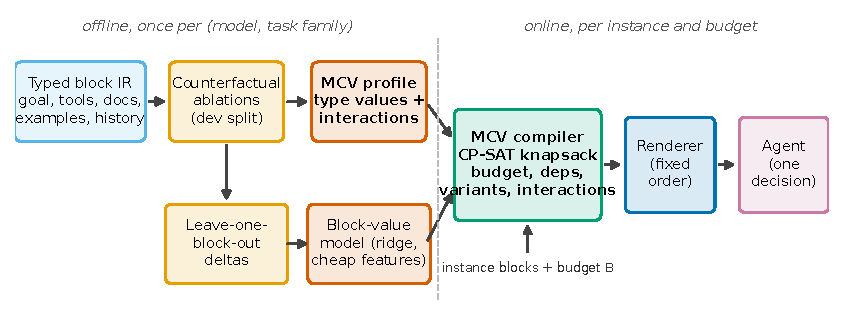
\includegraphics[width= 0.72\linewidth]{../figures/fig1_architecture.pdf}
\caption{MCV profiles and the MCV compiler. Profiling happens once per (model, task family) on development data;
compilation happens per instance and per budget without calling the language model (block embeddings are cached).}\label{fig:arch}
\end{figure}

\subsection{Typed Block IR and Rendering}
Each instance is converted by a deterministic adapter into typed blocks with full and, where meaningful, short variants
(a tool's name and description without its parameter schema; the first sentence of a document; the first sentence of a
history session). Rendering is a pure function of the selection: blocks appear in a fixed type order (instructions, tool
schemas, skill documents, examples, documents, notes, history in chronological order, and the goal last), so identical
selections yield byte-identical prompts and every policy in Section~\ref{sec:eval} is evaluated through the same renderer.
Token costs are measured with each model's own tokenizer.

\subsection{Profiling by Counterfactual Ablation}
For each development instance the profiler evaluates the full context and a set of ablations: every optional type
removed in turn; every pair of optional types removed; each type rendered with its short variant; and a sample of
single blocks removed (leave-one-block-out), which trains the instance-level model below. A length-neutral control
replaces a removed type with filler text of approximately equal token length, separating the effect of content from the effect of
prompt length. All runs use greedy decoding with a fixed seed and are cached by prompt hash, so repeated conditions cost
nothing.

\subsection{Estimation}
Type values, short-variant values and interaction terms are paired means over development instances (Definition~\ref{def:mcv}), each
shrunk toward zero by $n/(n+n_0)$ for $n$ instances, which damps cells measured on few instances, and reported with
paired percentile bootstrap intervals. Instance-level block values come from a ridge regression trained on the
leave-one-block-out deltas. Its features never use gold labels: block type, the type's MCV, the fraction of the goal's
content words that occur in the block, the block's BM25 rank within its type, log token length, for history its
recency, and the cosine similarity between block and goal embeddings. A short variant's value is the full value scaled by the type's measured ratio
$\mathrm{MCV}_{\mathrm{short}}(\tau)/\mathrm{MCV}(\tau)$, clipped to $[0,1]$.

\subsection{The MCV Compiler}
For instance $q$ and budget $B$ the compiler solves
\begin{align*}
\max\;&\textstyle\sum_{b,v}\hat v_{b,v}\,x_{b,v}+\sum_{\tau_1<\tau_2}I(\tau_1,\tau_2)\,y_{\tau_1\tau_2}\\
\text{s.t.}\;&\textstyle\sum_v x_{b,v}\le 1,\quad \sum_v x_{b,v}=1\ \text{for mandatory } b,\\
&\textstyle\sum_v x_{b,v}\le\sum_v x_{d,v}\ \ \forall d\in D_b,\\
&\textstyle\sum_{b,v}c(b,v)\,x_{b,v}\le B,\\
&z_\tau=\max_{b:\tau_b=\tau}\textstyle\sum_v x_{b,v},\quad y_{\tau_1\tau_2}=z_{\tau_1}z_{\tau_2},
\end{align*}
with binary variables, using the CP-SAT solver of OR-Tools under a time limit. Values are scaled to integers. The solver
returns a certificate (status, objective, bound, time); if no feasible solution is found in time, a value-density greedy
fills the budget and the certificate records the fallback. The additive objective never gains from a block with non-positive predicted value, so the compiler may leave budget
unused: more context is not assumed to be better. With interaction terms, a block of low or negative individual value
can still be selected when its type completes a positive interaction. The additive variant (OURS-A) drops
the interaction terms.

Appendix~\ref{app:compile} shows one compiled plan with its predicted block values, chosen variants and certificate.

\subsection{Transfer}
A profile measured on a small model is applied unchanged to a larger one (OURS-T). Fidelity is reported as the rank
correlation between the two models' type values and as the success difference between transferred and natively measured
profiles; the instance-level block-value model is shared, so the comparison isolates the type-level profile.

\section{Implementation}\label{sec:impl}
% IMPLEMENTATION. Numbers only via \R macros.
The reference implementation is the open-source Python package \texttt{mcv} (\RLoc{} lines; MIT license), with unit tests
covering the edge cases the design must handle: budgets smaller than the mandatory blocks (which raise an error rather than
truncating), dependency cycles and unknown dependencies, zero-value blocks, deterministic rendering order, the solver's
timeout path, and estimator recovery of known effects (\RTests{} tests, \RCoverage{} line coverage of the core
modules). Models run locally through Ollama with greedy decoding, a fixed seed and a fixed context window, so that the
model is never reloaded between conditions; models answer in a strict text protocol (a JSON call for tools, an
\texttt{ANSWER:} line otherwise) parsed by the harness. Responses are cached by a hash of (model, seed, decoding options,
prompt), so a prompt produced by several policies is answered once and the reuse is logged. Token costs use each model's
Hugging Face tokenizer, and the measured token count of every rendered prompt is logged so that budget compliance can be
audited. Embedding-based baselines use the open nomic-embed-text model~\citep{nomicembed2024} through the same server.
The compiler uses the CP-SAT solver of OR-Tools with a time limit per instance and a single worker for determinism.
Every run writes JSON-lines logs of each call, selection and solver certificate, plus a manifest with the code commit,
model digests and data hashes.\footnote{Software and data: Ollama \ROllamaVersion; OR-Tools, scikit-learn, LLMLingua and PyTorch
versions pinned in \texttt{code/uv.lock}; HotpotQA (CC BY-SA 4.0) and BFCL v3 (Apache-2.0) as recorded in
\texttt{data/LICENSES.md}.}

\section{Evaluation}\label{sec:eval}
% EVALUATION. Numbers ONLY via \R... macros from generated/numbers.tex.
\subsection{Setup}
\textbf{Task families.} Each family has \RNPerFamily instances, split once by a seeded shuffle into \RNDev development
and \RNTest test instances, with test hashes locked before any test run. \emph{Facts}: HotpotQA distractor questions
(validation split)~\citep{hotpotqa2018}; each instance carries its native paragraphs plus extra distractors drawn from other
questions (\RNumDocs documents, \RFullTokFacts tokens on average over all instances), two worked examples, and asks for a short answer.
\emph{Tool}: a call from the Berkeley Function Calling Leaderboard (BFCL v3) of the Gorilla project~\citep{gorilla2023} (simple and multiple categories); the
correct function or functions are mixed into a \RNumTools-tool catalog (\RFullTokTool tokens), and success is an
AST-level match of the emitted call. \emph{History}: \RNumSessions synthetic chat sessions (\RFullTokHistory tokens)
in which one user attribute is set and later updated, a knowledge-update setting also probed by
LongMemEval~\citep{longmemeval2024}; the agent must report the latest value, and in half of the
instances a note restates the \emph{stale} value. Success checks are deterministic.

\textbf{Models.} Qwen3-4B-Instruct-2507 (Ollama tag \texttt{qwen3:4b-instruct}, a non-thinking release) is the main
model and the profiling source; Qwen3-8B (tag \texttt{qwen3:8b}, the earlier hybrid-thinking release, run with thinking
disabled) is the transfer target, so transfer spans both model size and post-training release. Both are the default
4-bit Ollama builds (model digests in the run manifests) and run locally with greedy decoding, a fixed seed, a
\RNumCtx-token window and at most \RNumPredict output tokens.

\textbf{Policies.} B0 full context (no budget); B1 truncate oldest; B2 embedding relevance (nomic-embed-text cosine to
the goal, fill in descending order); B3 LLMLingua-2~\citep{llmlingua2_2024} compressing all optional context to the
remaining budget; B4 a PACMS-style facility-location coverage selector~\citep{pacms2026} (our re-implementation); B5 fixed
type tiers; OURS-A, the MCV compiler without interaction terms; OURS, with them. All policies keep the mandatory blocks
and share the renderer.

\textbf{Protocol.} Profiles use the first \RNProfFour development instances (4B, with \RNLobo leave-one-block-out samples
each) and \RNProfEight instances (8B, type level). Budgets are 1k, 2k, 4k and 8k tokens. The primary metric is the area
under the success--budget curve (AUBC), normalized over log-budget, per instance. The main grid evaluates B0, B2, B4,
OURS-A and OURS on the first \RNMain test instances per family; the weaker baselines B1, B3, B5 (well below B2 in dev
pilots) use the first \RNWeak. Following the pre-registration, H1 compares OURS with the best of B1--B5 per family; H1b
tests, at 8k, that OURS uses fewer tokens than B0 and the best baseline with success non-inferior to B0 (margin
\RMargin); H2 compares OURS with OURS-A pooled; H3 tests transfer. Intervals are paired percentile bootstraps
(\RNBoot resamples); p-values are Wilcoxon signed-rank for H1 and H2 and a one-sided paired bootstrap for H1b (the plan fixed the CI rule but named no test; recorded as a deviation); H1, H1b and H2
form one Holm family. All \RMainEpisodes main episodes completed. Block costs are summed in the model's tokenizer;
rendered prompts exceeded the budget in \ROverBudgetMain of \RBudgetedMain budgeted main-study episodes, by at most
\RMaxOvershoot tokens, because tokens merge at block boundaries.

\begin{table}[t]\centering\small
\caption{Test results on Qwen3-4B-Instruct: AUBC (mean, 95\% paired-bootstrap CI) and success at the 1k and 8k budgets.
B1, B3 and B5 use the first \RNWeak instances per family, the others \RNMain. B0 ignores the budget, so its 1k and 8k
entries are the same full-context run.}\label{tab:main}
\setlength{\tabcolsep}{2.6pt}
\fitwidth{%
\begin{tabular}{@{}l ccc ccc ccc@{}}\toprule
& \multicolumn{3}{c}{Facts (HotpotQA)} & \multicolumn{3}{c}{History (synthetic)} & \multicolumn{3}{c}{Tool (BFCL)}\\
\cmidrule(lr){2-4}\cmidrule(lr){5-7}\cmidrule(lr){8-10}
Policy & AUBC & @1k & @8k & AUBC & @1k & @8k & AUBC & @1k & @8k\\\midrule
B0 full & \RAubcFactsFull {\scriptsize[\RAubcFactsFullLo, \RAubcFactsFullHi]} & \RSucFullFacts & \RSucFullFacts & \RAubcHistoryFull {\scriptsize[\RAubcHistoryFullLo, \RAubcHistoryFullHi]} & \RSucFullHistory & \RSucFullHistory & \RAubcToolFull {\scriptsize[\RAubcToolFullLo, \RAubcToolFullHi]} & \RSucFullTool & \RSucFullTool\\
B1 truncate oldest & \RAubcFactsTrunc {\scriptsize[\RAubcFactsTruncLo, \RAubcFactsTruncHi]} & \RSucFactsTruncOne & \RSucFactsTruncEight & \RAubcHistoryTrunc {\scriptsize[\RAubcHistoryTruncLo, \RAubcHistoryTruncHi]} & \RSucHistoryTruncOne & \RSucHistoryTruncEight & \RAubcToolTrunc {\scriptsize[\RAubcToolTruncLo, \RAubcToolTruncHi]} & \RSucToolTruncOne & \RSucToolTruncEight\\
B2 relevance & \RAubcFactsRel {\scriptsize[\RAubcFactsRelLo, \RAubcFactsRelHi]} & \RSucFactsRelOne & \RSucFactsRelEight & \RAubcHistoryRel {\scriptsize[\RAubcHistoryRelLo, \RAubcHistoryRelHi]} & \RSucHistoryRelOne & \RSucHistoryRelEight & \RAubcToolRel {\scriptsize[\RAubcToolRelLo, \RAubcToolRelHi]} & \RSucToolRelOne & \RSucToolRelEight\\
B3 LLMLingua-2 & \RAubcFactsLingua {\scriptsize[\RAubcFactsLinguaLo, \RAubcFactsLinguaHi]} & \RSucFactsLinguaOne & \RSucFactsLinguaEight & \RAubcHistoryLingua {\scriptsize[\RAubcHistoryLinguaLo, \RAubcHistoryLinguaHi]} & \RSucHistoryLinguaOne & \RSucHistoryLinguaEight & \RAubcToolLingua {\scriptsize[\RAubcToolLinguaLo, \RAubcToolLinguaHi]} & \RSucToolLinguaOne & \RSucToolLinguaEight\\
B4 coverage (PACMS-style) & \RAubcFactsCov {\scriptsize[\RAubcFactsCovLo, \RAubcFactsCovHi]} & \RSucFactsCovOne & \RSucFactsCovEight & \RAubcHistoryCov {\scriptsize[\RAubcHistoryCovLo, \RAubcHistoryCovHi]} & \RSucHistoryCovOne & \RSucHistoryCovEight & \RAubcToolCov {\scriptsize[\RAubcToolCovLo, \RAubcToolCovHi]} & \RSucToolCovOne & \RSucToolCovEight\\
B5 type tiers & \RAubcFactsTier {\scriptsize[\RAubcFactsTierLo, \RAubcFactsTierHi]} & \RSucFactsTierOne & \RSucFactsTierEight & \RAubcHistoryTier {\scriptsize[\RAubcHistoryTierLo, \RAubcHistoryTierHi]} & \RSucHistoryTierOne & \RSucHistoryTierEight & \RAubcToolTier {\scriptsize[\RAubcToolTierLo, \RAubcToolTierHi]} & \RSucToolTierOne & \RSucToolTierEight\\
OURS-A (MCV additive) & \RAubcFactsAdditive {\scriptsize[\RAubcFactsAdditiveLo, \RAubcFactsAdditiveHi]} & \RSucFactsAdditiveOne & \RSucFactsAdditiveEight & \RAubcHistoryAdditive {\scriptsize[\RAubcHistoryAdditiveLo, \RAubcHistoryAdditiveHi]} & \RSucHistoryAdditiveOne & \RSucHistoryAdditiveEight & \RAubcToolAdditive {\scriptsize[\RAubcToolAdditiveLo, \RAubcToolAdditiveHi]} & \RSucToolAdditiveOne & \RSucToolAdditiveEight\\
OURS (MCV + interactions) & \RAubcFactsOurs {\scriptsize[\RAubcFactsOursLo, \RAubcFactsOursHi]} & \RSucFactsOursOne & \RSucFactsOursEight & \RAubcHistoryOurs {\scriptsize[\RAubcHistoryOursLo, \RAubcHistoryOursHi]} & \RSucHistoryOursOne & \RSucHistoryOursEight & \RAubcToolOurs {\scriptsize[\RAubcToolOursLo, \RAubcToolOursHi]} & \RSucToolOursOne & \RSucToolOursEight\\
\bottomrule\end{tabular}}
\end{table}

\begin{figure}[t]\centering
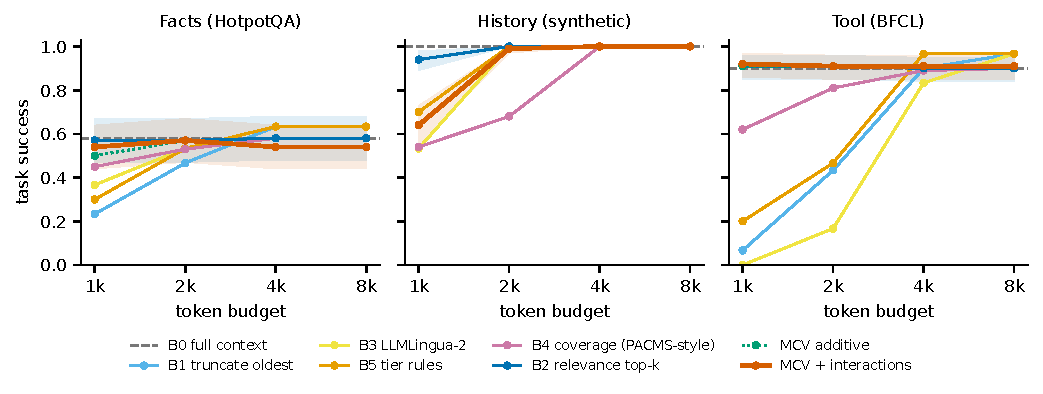
\includegraphics[width= 0.88\linewidth]{../figures/fig2_success_budget.pdf}
\caption{Success versus token budget on Qwen3-4B-Instruct (test). Bands: 95\% bootstrap CIs for B2 and OURS. The
dashed line is full context. MCV additive and MCV with interactions overlap almost everywhere.}\label{fig:curves}
\end{figure}

\begin{table}[t]\centering\small
\caption{Pre-registered hypotheses. Differences are paired (OURS minus comparator); H1 and H2 in AUBC, H1b and H3 in
success. $p$: Holm-adjusted over H1, H1b and H2 (two-sided Wilcoxon for H1 and H2, one-sided paired bootstrap for H1b);
H3 is decided by its CI against the margin \RMargin. Its interval is degenerate because transferred and native profiles
gave identical outcomes in every pair, so H3 passes without being informative (see the transfer results below).}\label{tab:hyp}
\setlength{\tabcolsep}{3pt}
\begin{tabular}{@{}llccl@{}}\toprule
Hyp. & Family & Difference [95\% CI] & $p$ & Outcome\\\midrule
H1 & Facts & \RHOneFactsDiff{} [\RHOneFactsLo, \RHOneFactsHi] & \RHOneFactsP & no gain\\
H1 & History & \RHOneHistoryDiff{} [\RHOneHistoryLo, \RHOneHistoryHi] & \RHOneHistoryP & worse\\
H1 & Tool & \RHOneToolDiff{} [\RHOneToolLo, \RHOneToolHi] & \RHOneToolP & no gain\\
H1b & Facts & \RHOnebFactsDiff{} [\RHOnebFactsLo, \RHOnebFactsHi] & \RHOnebFactsP & not shown\\
H1b & History & \RHOnebHistoryDiff{} [\RHOnebHistoryLo, \RHOnebHistoryHi] & \RHOnebHistoryP & non-inferior\\
H1b & Tool & \RHOnebToolDiff{} [\RHOnebToolLo, \RHOnebToolHi] & \RHOnebToolP & non-inferior\\
H2 & Pooled & \RHTwoPooledDiff{} [\RHTwoPooledLo, \RHTwoPooledHi] & \RHTwoPooledP & no effect\\
H3 & Pooled & \RTransferDiff{} [\RTransferLo, \RTransferHi] & -- & \RHThreeVerdict{}$^{*}$\\
\bottomrule\end{tabular}
\end{table}

\subsection{Main Result: H1 Is Not Supported}
Table~\ref{tab:hyp} summarizes all pre-registered tests. 
Table~\ref{tab:main} and Fig.~\ref{fig:curves} give the main comparison. Embedding relevance (B2) was the best baseline
in every family. OURS did not exceed it anywhere: the paired AUBC difference was \RHOneFactsDiff{}
[\RHOneFactsLo, \RHOneFactsHi] on facts and \RHOneToolDiff{} [\RHOneToolLo, \RHOneToolHi] on tool use, both
indistinguishable from zero, and \RHOneHistoryDiff{} [\RHOneHistoryLo, \RHOneHistoryHi] on history, a significant
\emph{loss} (Holm $p\RHOneHistoryPRel$). H1 required a significant gain in two families; it fails.

On tool use the MCV compiler beat the non-relevance baselines by wide margins at small budgets: at 1k it reached
\RSucToolOursOne success against \RSucToolLinguaOne for LLMLingua-2, \RSucToolTruncOne for truncation and
\RSucToolCovOne for coverage, because it spends the budget on the tool schemas ranked most valuable and often drops
examples. This advantage did not hold elsewhere: on history at 1k OURS (\RSucHistoryOursOne) trailed truncation
(\RSucHistoryTruncOne) and tiers (\RSucHistoryTierOne). Relevance ranking also concentrates the budget on goal-related blocks. Once a block's value is dominated by
whether it is about the goal, an embedding score already captures most of what the profile adds.

\textbf{Diagnosis of the history loss.} Almost all of the history gap arises at the 1k budget (at 2k and above both policies
are at or near ceiling). There, success depends almost only on whether the session containing the latest update
survives selection. OURS kept it in \RRecallOurs of plans and B2 in \RRecallRel; without that session OURS never
answered correctly (\RSucGivenNoGoldOurs). Two causes combine. The first is the block-value model. Trained on
leave-one-block-out deltas, its history coefficients (unstandardized; recency spans the unit interval, while goal similarity varies over a narrow range) weight recency (\RCoefRecency) and token length
(\RCoefLen) alongside embedding similarity (\RCoefSim), so it fills a small budget with the most recent sessions and
misses the update whenever it lies further back. The second is the profile itself, applied far from where it was
measured. The note's value (\RMcvHistoryNote) is a leave-one-type-out effect from the full context, where history already
supplies the answer, and the interaction term penalizes sending both. At 1k, OURS sent the note in \RNoteInOursOne of
plans, against \RNoteInRelOne for relevance, so when the update session was dropped no fallback remained. In an
exploratory check of the logs (not pre-registered), \ROursFailCurrentNote of the \ROursFailHistOne OURS failures at 1k
were instances whose note held the \emph{current} value, and policies that kept a current note but missed the update
session answered correctly in \RNoteRescueRate of \RNoteRescueN such episodes. A type value measured at full context is
therefore not a valid value at a small budget for types that are redundant only in the presence of others. The
leave-one-block-out signal is sparse: removing one of \RNumSessions sessions rarely changes the outcome, so the
regression learns weak correlates of value instead of value. An exploratory check on the development logs confirms this (not
pre-registered; five-fold cross-validation grouped by instance). Only \RCvNonzeroHistory of history-session deletions
changed the outcome (\RCvNonzeroFacts for documents, \RCvNonzeroTool for tool schemas). The cross-validated rank
correlation between predicted and observed deltas was \RCvModelHistory for the ridge model against \RCvSimHistory for
embedding similarity alone on history, \RCvModelFacts against \RCvSimFacts on facts, and \RCvModelTool for both on
tool use. The learned ranker was never better than its own similarity feature.

\subsection{Pruning: H1b Is Supported in Two of Three Families}
Because the compiler adds blocks only while they raise the predicted objective, it leaves budget unused at 8k
(Fig.~\ref{fig:composition}), whereas B2 fills the budget and so matches full context. On tool use OURS sent
\RTokOursTool tokens instead of \RTokFullTool (\RTokCutTool fewer) with success \RSucOursEightTool against
\RSucFullTool for full context (difference \RHOnebToolDiff, CI [\RHOnebToolLo, \RHOnebToolHi], Holm
$p\RHOnebToolPRel$). On history it sent \RTokCutHistory fewer tokens with identical success (\RSucOursEightHistory),
the saving coming from the examples, the note and a few low-value sessions. On facts it sent \RTokCutFacts fewer tokens,
but success fell from \RSucFullFacts to \RSucOursEightFacts and the CI [\RHOnebFactsLo, \RHOnebFactsHi] crosses the
margin, so non-inferiority is not shown there. Two families pass, as H1b required. Two caveats bound this result. Full contexts average \RFullTokFacts, \RFullTokHistory
and \RFullTokTool tokens, so the 8k budget never binds (nor does 4k except on tool use). H1b therefore tests pruning of
full context, not selection under a binding budget. The savings come from the block-level values, which stop adding
blocks once predicted value reaches zero; the follow-up below shows that relevance with a stopping rule achieves them
without MCV. On facts, full context was right and
OURS wrong on \RFactsLost instances, and the reverse held on \RFactsGained. Only \RFactsLostGoldDropped of those losses
removed a supporting paragraph; in the others the model changed its answer when distractors were removed, an effect a
type-level profile cannot see.


\begin{figure}[t]\centering
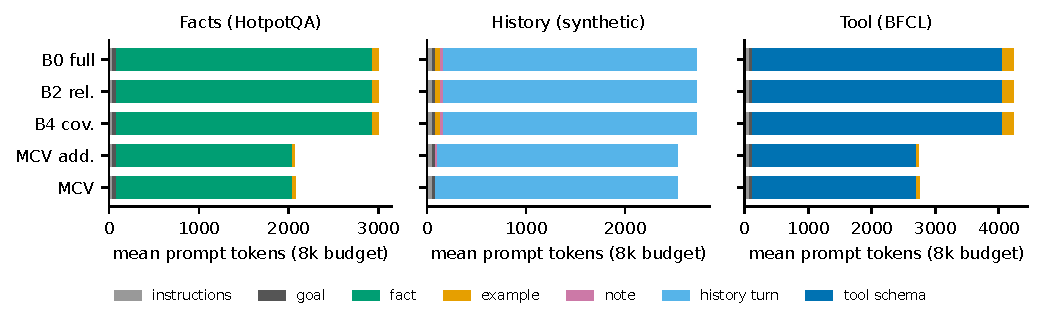
\includegraphics[width= 0.88\linewidth]{../figures/fig5_composition.pdf}
\caption{Mean prompt composition at the 8k budget (test, Qwen3-4B-Instruct). MCV leaves budget unused: it drops the
profile note, most low-value documents and tool schemas, and some worked examples.}\label{fig:composition}
\end{figure}

\subsection{Interactions: H2 Has No Detectable Effect}
Adding interaction terms changed pooled AUBC by \RHTwoPooledDiff{} [\RHTwoPooledLo, \RHTwoPooledHi] (Holm
$p\RHTwoPooledPRel$). History is at ceiling from 2k upward, which leaves little room for any difference, so this null result is limited. The
only large interaction measured is between history and the profile note (\RIntHistoryHistoryTurnNote). Because the note
is current in half of the instances and stale in the other half, the negative sign means the two substitute for each
other: either can supply the answer when it is current, and the note adds nothing once history is present (its own
value is \RMcvHistoryNote). The interaction terms did change the plans: OURS and OURS-A
selected different blocks in \RSelDiffFacts of facts, \RSelDiffHistory of history and \RSelDiffTool of tool plans.
At 8k, OURS never included the note while OURS-A included it in \RHasNoteAdditiveHistory of history plans, and the
positive example--document interaction (\RIntFactsExampleFact) made OURS keep an example in \RHasExampleOursFacts of
facts plans against \RHasExampleAdditiveFacts for OURS-A. These changes concern low-value blocks and rarely changed
success (\RSelOutcomeDiffFacts, \RSelOutcomeDiffHistory and \RSelOutcomeDiffTool of episodes). On these families, type-pair interactions change what is sent but not whether the task succeeds.

\subsection{Post-hoc Follow-up: Stopping Rules and a Hybrid}
The results above leave two questions open: are the token savings specific to MCV, and does the three-level split of
Section~\ref{sec:problem} help if each level uses the signal that worked? After the main results were known we
pre-specified a follow-up (an addendum to the pre-registration, committed before any of its runs) with two policies.
\emph{B2S} is relevance ranking with a stopping rule: blocks whose goal cosine falls below a threshold $\tau$ are never
added. \emph{HYB} is a hybrid: the 4B profile admits only types whose MCV interval excludes zero (documents, history
sessions, tool schemas), relevance ranks blocks within admitted types with value $\cos-\tau$, and the compiler applies the
budget, dependencies and short variants. Each family's $\tau$ was chosen from a five-point grid on \RNCalib development
instances not used for profiling, as the most token-saving value whose success at 8k stayed within \RMargin of full
context. The same rule picked the same $\tau$ for both policies in every family. Both were run on the main test instances
and budgets; H6 tests B2S and H8 tests HYB for non-inferiority to full context at 8k, H7 tests HYB against B2 in AUBC
(one Holm family of nine tests).

\begin{table}[t]\centering\small
\caption{Post-hoc follow-up (test, Qwen3-4B-Instruct, \RNMain instances per family). AUBC; success and prompt-token
reduction relative to full context at 8k. Non-inferiority margin \RMargin.}\label{tab:followup}
\setlength{\tabcolsep}{3pt}
\fitwidth{%
\begin{tabular}{@{}lccc@{}}\toprule
 & Facts & History & Tool\\\midrule
AUBC: B2 / OURS & \RAubcFactsRel{} / \RAubcFactsOurs & \RAubcHistoryRel{} / \RAubcHistoryOurs & \RAubcToolRel{} / \RAubcToolOurs\\
AUBC: B2S / HYB & \RAubcFactsStop{} / \RAubcFactsHyb & \RAubcHistoryStop{} / \RAubcHistoryHyb & \RAubcToolStop{} / \RAubcToolHyb\\
H7: HYB$-$B2 [CI] & \RHSevenFactsDiff{} {\scriptsize[\RHSevenFactsLo, \RHSevenFactsHi]} & \RHSevenHistoryDiff{} {\scriptsize[\RHSevenHistoryLo, \RHSevenHistoryHi]} & \RHSevenToolDiff{} {\scriptsize[\RHSevenToolLo, \RHSevenToolHi]}\\\midrule
@8k success: B0 / OURS & \RSucFullFacts{} / \RSucOursEightFacts & \RSucFullHistory{} / \RSucOursEightHistory & \RSucFullTool{} / \RSucOursEightTool\\
@8k success: B2S / HYB & \RSucFactsStopEight{} / \RSucFactsHybEight & \RSucHistoryStopEight{} / \RSucHistoryHybEight & \RSucToolStopEight{} / \RSucToolHybEight\\
@8k tokens cut: OURS & \RTokCutFacts & \RTokCutHistory & \RTokCutTool\\
@8k tokens cut: B2S / HYB & \RTokCutStopFacts{} / \RTokCutHybFacts & \RTokCutStopHistory{} / \RTokCutHybHistory & \RTokCutStopTool{} / \RTokCutHybTool\\
H6: B2S$-$B0 [CI] & \RHSixFactsDiff{} {\scriptsize[\RHSixFactsLo, \RHSixFactsHi]} & \RHSixHistoryDiff{} {\scriptsize[\RHSixHistoryLo, \RHSixHistoryHi]} & \RHSixToolDiff{} {\scriptsize[\RHSixToolLo, \RHSixToolHi]}\\
\bottomrule\end{tabular}}
\end{table}

Table~\ref{tab:followup} gives the results. \textbf{The hybrid did not improve selection.} HYB exceeded B2 in none of the
three families (H7; Holm-adjusted $p$ \RHSevenFactsP, \RHSevenHistoryP and \RHSevenToolP), and its AUBC was close to that of OURS
(HYB$-$OURS: \RHybVsOursFacts, \RHybVsOursHistory, \RHybVsOursTool). On history its bootstrap interval against B2 lies
entirely below zero (\RHSevenHistoryDiff{} [\RHSevenHistoryLo, \RHSevenHistoryHi]), although the Wilcoxon test is not
significant: its calibrated threshold sometimes excludes the update session itself, at every budget, the same loss
B2S shows on history. \textbf{The type filter added nothing measurable here:} HYB and
B2S produced the same outcome in \RHybStopSame of episodes, although B2S kept an example or the note in most of its plans. This
is consistent with the profiles: the excluded types carry little value, so removing them saves some tokens
(\RTokCutHybTool against \RTokCutStopTool on tool use) without changing outcomes. \textbf{The savings are not specific to MCV.} On tool use,
relevance with a stopping rule was non-inferior to full context at 8k (H6, Holm $p\RHSixToolPRel$) while removing
\RTokCutStopTool of prompt tokens, against \RTokCutTool for OURS; HYB behaved alike (H8, $p\RHEightToolPRel$). On facts and
history the calibrated thresholds were too aggressive for the test set: they removed \RTokCutStopFacts and
\RTokCutStopHistory of tokens, but success fell by \RHSixFactsDiff{} and \RHSixHistoryDiff{}, and non-inferiority was not
shown. There, the more conservative OURS kept success at the cost of smaller savings. A threshold calibrated on
\RNCalib instances is a coarse instrument; the facts calibration curve was not even monotone. On tool use the rule chose the
largest threshold in the grid, so the saving reported there is a lower bound on what a stopping rule could remove.

\subsection{What the Profiles Say}
Fig.~\ref{fig:profiles} and Table~\ref{tab:profiles} show the profiles of both models. Three regularities hold across families. First,
the value of context is concentrated: tool schemas (\RMcvToolToolSchema), documents (\RMcvFactsFact) and history
sessions (\RMcvHistoryHistoryTurn) carry nearly all of it. Second, worked examples are worth close to nothing
on their own (\RMcvFactsExample, \RMcvHistoryExample, \RMcvToolExample on the 4B model; the 8B model valued them
at \RMcvEightHistoryExample on history), although every family's prompt includes them by default. Third, short variants are worth much less than full blocks for tool schemas
(\RShortToolToolSchema against \RMcvToolToolSchema), because the parameter schema matters for argument filling.
The length-neutral control, which replaces a removed type with filler of approximately equal token length (\RPadN instances per
type), reproduced the removal effects: documents \RRemFactsFact by removal against \RPadFactsFact with padding, tool
schemas \RRemToolToolSchema against \RPadToolToolSchema, history \RRemHistoryHistoryTurn against
\RPadHistoryHistoryTurn. The measured values reflect content, not prompt length.


\begin{figure}[t]\centering
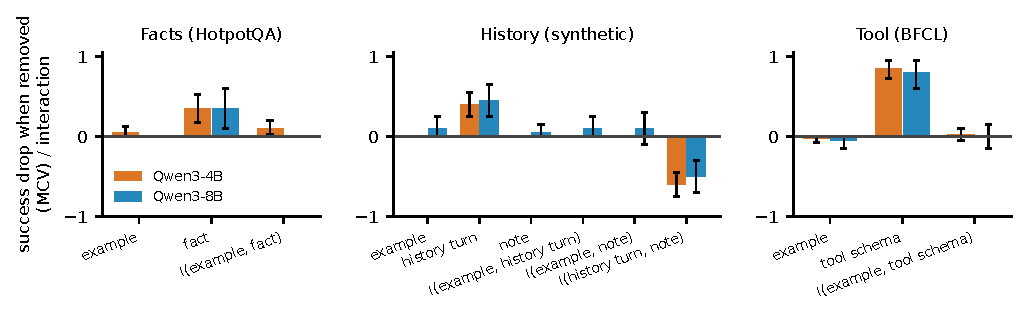
\includegraphics[width= 0.88\linewidth]{../figures/fig3_profiles.pdf}
\caption{MCV profiles (development split): success drop when a type is removed, and pairwise interactions
$I(\tau_1,\tau_2)$, for Qwen3-4B-Instruct (\RNProfFour instances) and Qwen3-8B (\RNProfEight instances), with 95\%
bootstrap CIs.}\label{fig:profiles}
\end{figure}

\subsection{Transfer Across Model Size and Release (H3)}
The 4B and 8B profiles rank the \RRhoN (family, type) values similarly (Spearman $\rho=\RRho$, pooled across families, so
between-family differences contribute to the agreement), and their magnitudes agree
closely (Fig.~\ref{fig:profiles}). On Qwen3-8B (first \RNTransfer test instances per family, budgets 2k and 8k),
compiling with the transferred 4B profile and with the natively measured 8B profile gave a pooled success difference of
\RTransferDiff{} [\RTransferLo, \RTransferHi] over \RTransferN paired episodes, so H3 non-inferiority holds
(Fig.~\ref{fig:transfer}). The outcome was the same in \RTransferAllEqual of paired episodes, giving the degenerate
interval above, although the two profiles
produced identical selections in only \RTransferSameSel. The differences involved tool schemas,
history sessions and examples alike, yet never changed the outcome. This suggests that both profiles keep the blocks
that decide success and differ only in blocks that do not. It equally indicates that, with the block-value model
shared, the compiler's outcomes are insensitive to the type-level profile, so H3 does not show that the profile drives
the decisions that matter. The efficiency pattern of the 4B study carried over. On tool use at 8k the transferred profile
sent \RTrTokToolTransferEight prompt tokens against \RTrTokToolRelEight for relevance ranking, with success
\RTrToolTransferEight against \RTrToolRelEight. Relevance ranking was again more accurate on facts (\RTrFactsRelTwo
against \RTrFactsTransferTwo at 2k). With \RNTransfer instances per family these 8B comparisons are descriptive.


\textbf{Failure analysis.} Transcripts show three failure modes: abstentions when the session holding an update is dropped, identifiers corrupted by LLMLingua-2 compression, and answer changes on facts even when all evidence was kept (Appendix~\ref{app:failures}).

\textbf{Profiling sample size.} In an exploratory subsampling analysis the type-level profile stabilized with ten to twenty development instances per family (Appendix~\ref{app:samplesize}).

\subsection{Cost}
\textbf{Compilation.} Over \RSolves compilations CP-SAT proved optimality in \RSolveOptimal of cases with no fallback
(\RSolveFallback); median solve time was \RSolveMedianMs{} ms (99th percentile \RSolveNinetyNineMs{} ms, maximum
\RSolveMaxMs{} ms), and end-to-end planning including feature computation (with cached block embeddings) took a median \RPlanMedianMs{} ms.
\textbf{Profiling.} The 4B profile cost \RProfCallsTotal model calls (\RProfHours hours on a laptop). Measured in
prompt tokens, profiling pays for itself after about \RBreakEvenTool queries on tool use and \RBreakEvenFacts on
facts, given the 8k-budget savings above. The facts figure is conditional on accepting that family's non-significant success loss. History saves less per query and breaks even after about
\RBreakEvenHistory.



\textbf{Development history.} The block-value model went through three development versions before the method was frozen and pre-registered; all are reported in Appendix~\ref{app:devhistory}.

\section{Discussion, Limitations and Threats to Validity}\label{sec:limits}
% DISCUSSION, LIMITATIONS AND THREATS TO VALIDITY. Numbers ONLY via \R... macros.
\subsection{What the Results Mean}
In these experiments measured context value was more useful for diagnosing which kinds of context matter than for
choosing individual blocks. At the block level, embedding relevance was hard to beat: neither the MCV compiler nor the
hybrid improved on it, and the learned block ranker was worse where it substituted recency for relevance. At the type
level, the profiles exposed structure that relevance scores do not report: value concentrated in one or two types per
family, worked examples with little individual value, a substitution between history and the note, and a large loss
from shortening tool schemas. The token savings came from not sending context, and a relevance ranker with a stopping
rule achieved them as well, so they are a property of stopping rather than of MCV.

The block-level failure is informative about supervision. When many blocks are individually dispensable (one session of
\RNumSessions, one document of \RNumDocs), single deletions rarely change the outcome, and a regression on those deltas
learns proxies. Group or pairwise deletions, or relevance itself as the within-type ranker, are the natural fixes; the
hybrid tested the latter and matched relevance with a stopping rule almost exactly.

\subsection{Design Lesson and Future Work}
The evidence suggests separating type-level valuation from instance-level relevance: a type profile decides which
types deserve budget and flags low-value or redundant context; relevance ranks blocks within types; a stopping rule or
constraint-aware compiler decides when more context is not worth sending. Our hybrid instantiated this pipeline and did
not beat relevance on these families, where the excluded types already had little effect on outcomes. Whether the type
level helps where low-value types are large, numerous or harmful remains untested. Three experiments would most
strengthen these conclusions: (i) stopping thresholds calibrated on a larger development set, since our calibration on
\RNCalib instances per family was too aggressive for facts and history; (ii) the same protocol on a model family other
than Qwen, which would test whether profiles and the null selection result generalize; and (iii) tasks with binding
budgets and long-horizon trajectories, where type-level allocation has more room to matter.

\subsection{Practical Guidance}
The results suggest a cheap procedure. Profile each (model, task family) on a small development set (ten to twenty
instances sufficed here to rank types, judged from subsamples of the same \RNProfFour instances), using type removals and
the length-neutral control. Use the profile to audit the default prompt: consider removing types whose value interval sits
at zero (here, worked examples on history and tool use) after checking their interactions. Rank blocks by relevance, and
calibrate a stopping threshold on held-out development data rather than filling the budget. Re-profile when the model or
task family changes. Interaction terms can be omitted unless two valuable types interact strongly.

\subsection{Limitations and Threats to Validity}
\textbf{Construct validity.} Each instance is a single agent decision, not a multi-step trajectory with a simulated
user as in $\tau$-bench~\citep{taubench2024}; context value in long-horizon agents may compound across steps. Success is a deterministic check (answer match, AST-level call match),
which misses partially correct outputs.
\textbf{Internal validity.} B4 is our re-implementation of a PACMS-style objective, not the authors' code, and B3 uses one
LLMLingua-2 checkpoint; both could be tuned further. Rendered prompts may exceed the budget by at most \RMaxOvershoot
tokens because tokenization is not additive across block boundaries. Reading transcripts after the test runs revealed a defect in the tool checker: it compared list-valued arguments as
strings, so an integer list failed against the same values written as floats. Rescoring all logged answers with
element-wise numeric comparison changed \RCheckerFlips episodes, spread across all policies, and left the H1, H1b and H2
mean paired differences unchanged at three decimals (for example H1 on tool use, \RSensHOneTool). We keep the
pre-registered checker as primary. Greedy decoding on Apple-silicon inference is not
guaranteed to be bitwise deterministic; caching makes every reported response reproducible from the logs, but a fresh
rerun may differ slightly.
\textbf{Statistical conclusion validity.} The pre-registered power analysis put power for a \RSesoi{} AUBC effect on facts at
about \RPowerFacts with \RNMain instances, so the null result on facts is weak evidence of no effect. The weaker baselines used
\RNWeak instances; each scored below B2 in every family (Table~\ref{tab:main}), so B2 is the best baseline throughout. Transfer used
\RNTransfer instances per family and two budgets. The follow-up (B2S, HYB) was specified after the main results were
known and reuses the same test instances; its thresholds were calibrated on \RNCalib development instances per family,
which proved noisy.
\textbf{External validity.} Two models of one family (Qwen3, 4B and 8B) were tested; a third model from another family
was planned and dropped for compute, so neither the profiles nor transfer are shown to generalize beyond Qwen3. Identical paired outcomes under transferred
and native profiles, despite differing selections, cannot distinguish faithful transfer from compiler insensitivity. One task family (history) is
synthetic; HotpotQA is known to admit reasoning shortcuts that MuSiQue was built to remove~\citep{musique2022}; and
HotpotQA and BFCL may overlap with pretraining data. Profiles are per (model, task family) and must be
re-measured when either changes, at the profiling cost reported in Section~\ref{sec:eval}.

\section{Conclusion}\label{sec:conclusion}
% CONCLUSION. Numbers ONLY via \R... macros.
We asked whether measuring how much each type of context contributes to task success can be reused for budgeted
context assembly. In these experiments, measured context value was more useful for diagnosing which kinds of context
matter than for ranking individual blocks. Embedding relevance remained difficult to beat at the instance level: neither
the MCV compiler nor a hybrid built on the profile improved on it, and supervision from single-block deletions was too
sparse to learn block value. Type-level ablations nevertheless exposed concentrated, redundant and low-value context,
and the largest token savings came from deciding when to stop sending context. These results motivate context-assembly
designs that keep type-level valuation and block-level relevance separate, and we release every log so that the
negative results can be checked and extended.

\textbf{Use of AI assistance.} An AI coding assistant was used to write and test code, run the experiments, and draft
and edit text. All numbers in the paper are generated from the released logs by scripts, and every reference was
verified against its DOI record. The author reviewed the content and is responsible for it.

\textbf{Artifact availability.} The \texttt{mcv} package, data adapters (with the licenses of HotpotQA and BFCL),
pre-registration, raw logs of every model call, and the scripts that regenerate all figures, tables and numbers with one
command will be released under an open license with the preprint.


\bibliography{references}
\bibliographystyle{tmlr}
\end{document}
